 
% !TeX spellcheck = pl_PL
\documentclass[]{article}
\usepackage[polish]{babel}
\usepackage[utf8]{inputenc}
\usepackage[T1]{fontenc}
\usepackage{array}
\usepackage{amsmath}
\usepackage{graphicx}
\usepackage{multirow}
\usepackage{makecell}
\usepackage{geometry}
\graphicspath{{./images/}}

\author{Jakub Gosławski 141222 jakub.goslawski@student.put.poznan.pl 
\and Michał Wiśniewski 141355 michal.janu.wisniewski@student.put.poznan.pl}
\date{22 listopada 2019}
\title{Sprawozdanie z laboratorium Optymalizacji Kombinatorycznej: 
\newline Problem Job-shop wykonany metodą wielokrotnego wspinania się (hill climbing)}

\newgeometry{vmargin={25mm}, hmargin={25mm}}

\begin{document}
	\maketitle
	
	\section{Implementacja}
	Implementacja problemu została wykonana obiektowo w języku C++.
	Kod dzieli się na trzy zasadnicze części, interpretację plików wejściowych, algorytm wyznaczający nowe rozwiązanie oraz algorytm optymalizacyjny wybierający i analizujący rozwiązania metodą wielokrotnego wspinania się (Hill Climbing).
	
	\begin{figure}[h!]
		\centering
		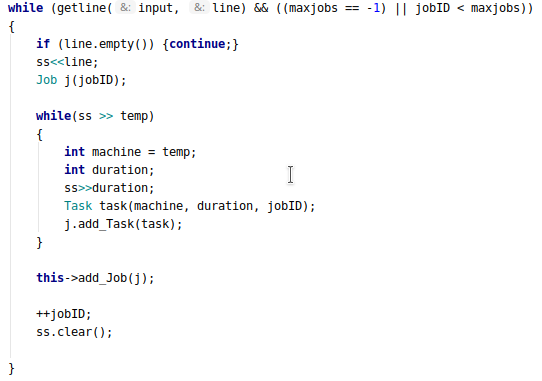
\includegraphics[width=0.5\linewidth]{orlib}
		\caption{Interpretacja danych instancji typu orlib}
	\end{figure}

	Obiekt Factory (fragment konstruktora przedstawiony powyżej) składa się z obiektów Job, które składają się z obiektów Task, wszystkie przechowywane w wektorach, aby zachować kolejność przedstawioną w pliku wejściowym.\\
	
	
	\begin{figure}[h!]
		%\centering
		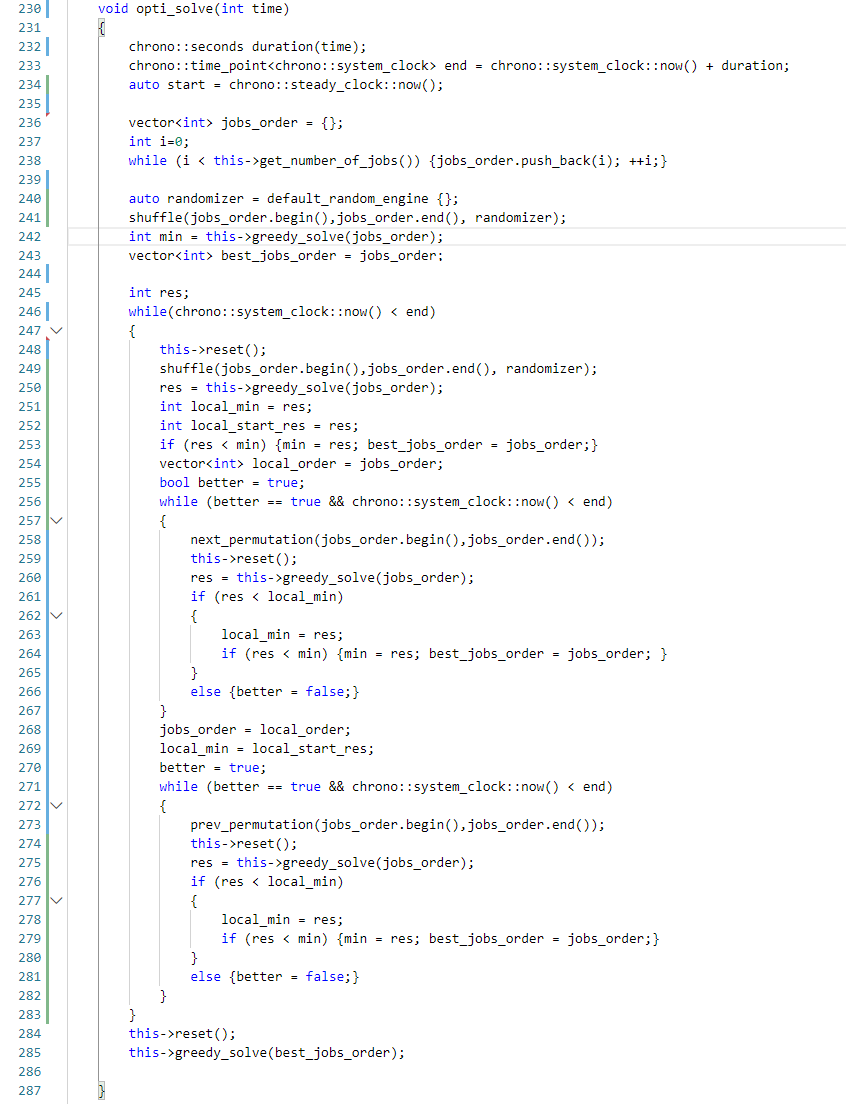
\includegraphics[width=1\linewidth]{greedy}
		\caption{Algorytm optymalizacyjny}
	\end{figure}

	Algorytm wyznaczający nowe rozwiązanie to zmodyfikowana wersja algorytmu zachłannego, który za parametr przyjmuję permutację zadań (Jobs) i według niej przypisuje kolejne zadania (Tasks). 
	Algorytm optymalizacyjny rozpoczyna się włączeniem pomiaru czasu i wygenerowaniem pierwszego rozwiązania na podstawie wcześniej wylosowanej permutacji. Następnie generowana jest następna wg porządku leksykograficznego permutacja zadań, i dopóki wynik rozwiązania się ulepsza, tak długo dokonuje kolejnych prób z następnymi permutacjami i przyjmuje je jako lokalne maksimum. Następnie algorytm wraca do pierwotnie wylosowanej permutacji i porusza się tym razem w drugą stronę (generując poprzednie wg porządku leksykograficznego permutacje zadań), tak długo jak wynik będzie się ulepszał. O ile upłynięty czas jest krótszy aniżeli ten z argumentu funkcji algorytmu, zostaje wygenerowane nowe losowe rozwiązanie i względem niego powtarzane są powyższe kroki wpisania się w obie strony. Ponieważ generowanie nowych fabryk przy każdym rozwiązaniu wiązałoby się z ogromną złożonością pamięciową, algorytm optymalizacyjny pracuje na jednej wczytanej fabryce i przed kolejnym rozwiązaniem wywoływana jest funkcja resetująca.
	Do pomiaru bieżącego czasu wykorzystywany jest system\_clock z biblioteki std::chrono. Losowanie wykorzystuje funkcję shuffle oraz deflaut\_radnom\_engine z biblioteki <random>, a przemieszanie się po kolejnych permutacjach funkcje next\_permutation i prev\_permutation z biblioteki <algorithm>.
	
	
	\subsection{Użycie}
	
	 Program wykonuje się z linii poleceń i przyjmuje parametry: nazwa pliku, format instancji (o - orlib, t -tailard), oraz opcjonalną liczbę wczytanych pierwszych zadań, a zapisuje rozwiązanie w nowym pliku o nazwie [nazwa instancji]\_answer.txt. 
	
	\section{Testy}
	\subsection{Testy jakości}
	

	
	
	\subsection{Testy jakości w zależności od czasu}
		
	Testy czasu wykorzystywały klasę high\_resolution\_clock z biblioteki std::chrono i mierzyły czas z dokładnością 1 nanosekundy.
	
	\begin{figure}[h!]
		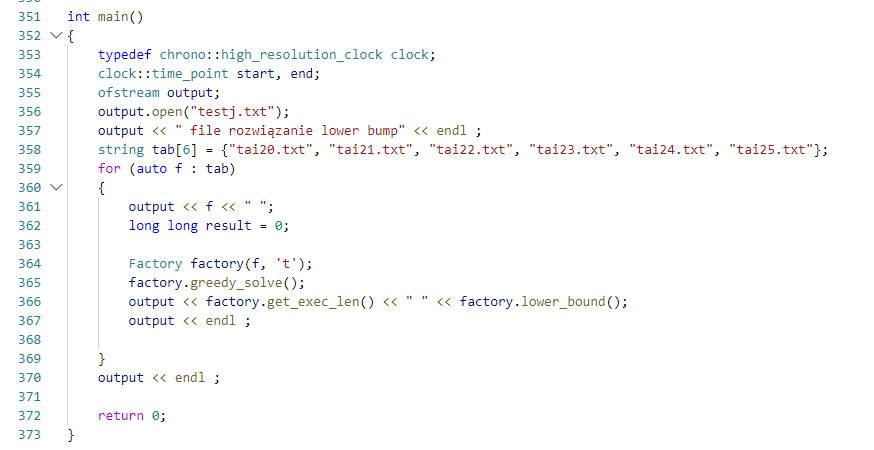
\includegraphics[width=\linewidth]{kod_testy_jakosci}
		\caption{Kod użyty do wyznaczenia pomiarów jakościowych}
	\end{figure}

	\begin{table}[h!]
		\centering
		\caption{Testy jakości rozwiązań dla instancji tai20-25}
		\begin{tabular}{|l|l|l|}
			\hline
			
			Instancja & Wynik & Wyznaczony lower bump \\ \hline
			tai20 & 2360 & 928 \\ \hline
			tai21 & 2308 & 1217 \\ \hline
			tai22 & 2567 & 1223 \\ \hline
			tai23 & 2282 & 1164 \\ \hline
			tai24 & 2487 & 1151 \\ \hline
			tai25 & 2566 & 1170 \\ \hline
			
		\end{tabular}
	\end{table}
	
	\begin{figure}%[h!]
		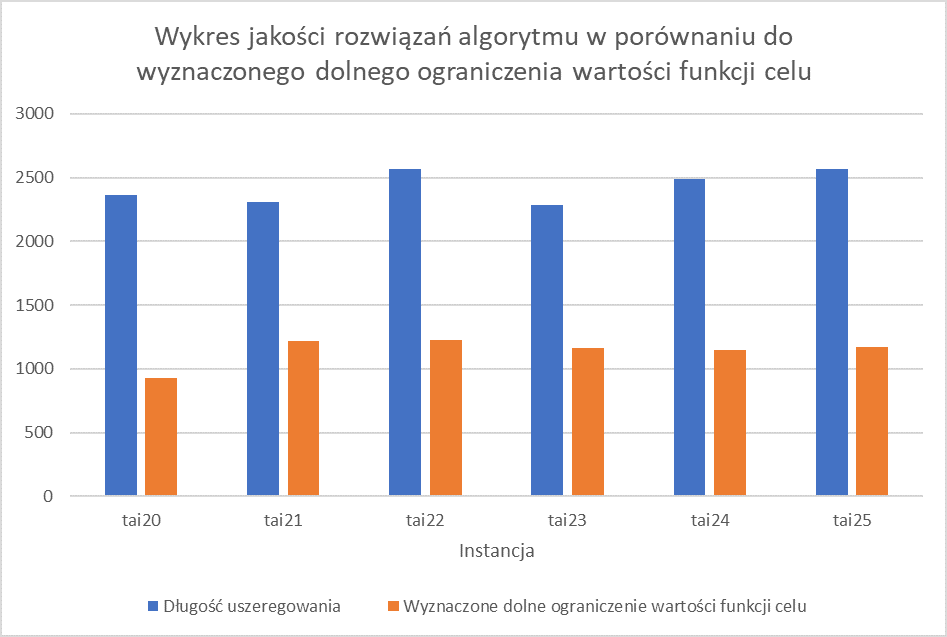
\includegraphics[width=\linewidth]{wykres3}
	\end{figure}
	
\end{document} 
